\section{Results}
	Even with not bad accuracy of 73.52\% at first attempt it was worth to check confusion matrix to target low accuracy classification results.
	
	\begin{figure}[H]
        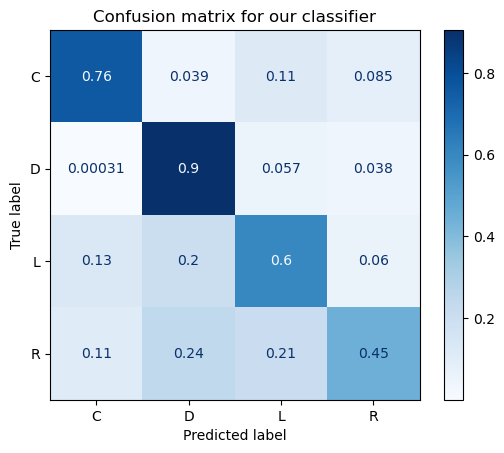
\includegraphics[width=0.6\textwidth]{matrix}
    \end{figure}
	
	\begin{itemize}
		\item the highest accuracy is for defence (D) players it's 90\% there would probably be not much space for optimization here
		\item center position (C) has 76\% accuracy it can be optimized a little to achieve better accuracy
		\item the two worst cases are left wing (L) and right wing (R) players for whom accuracy is 60\% and 45\%
	\end{itemize}
	
	\section{Discussion}
	\begin{itemize}
		\item what stands opposite to domain knowledge is that there is about 20\% probability of classifying wing players as defence players, stats of players from one line should be similar and thus probability of false positives should appear between those positions
		\item it's worth checking whether model could be optimized by dropping some of the player data from training set, especially the ones that for example have time on ice lower then average of other players at that position
		\item from the model it follows that defence players statistics vary significantly from centre and wing players thus accuracy for defence is very high
		
	\end{itemize}

	\textbf{github repository link:}
	\href{https://github.com/saigupta001/Team\_Coders}{https://github.com/saigupta001/Team\_Coders}
